\subsection{Results}

The reconstruction method was experimented both on synthetical data and real
clinical data. Compared with real data, the reconstruction of synthetical
data is easy to assess because of knowing the vessel ground truth. The final
reconstruction results of synthetical data can be found in Figure
\ref{fig:experiments_full}.

\begin{figure*}
  \centering
  % Requires \usepackage{graphicx}
  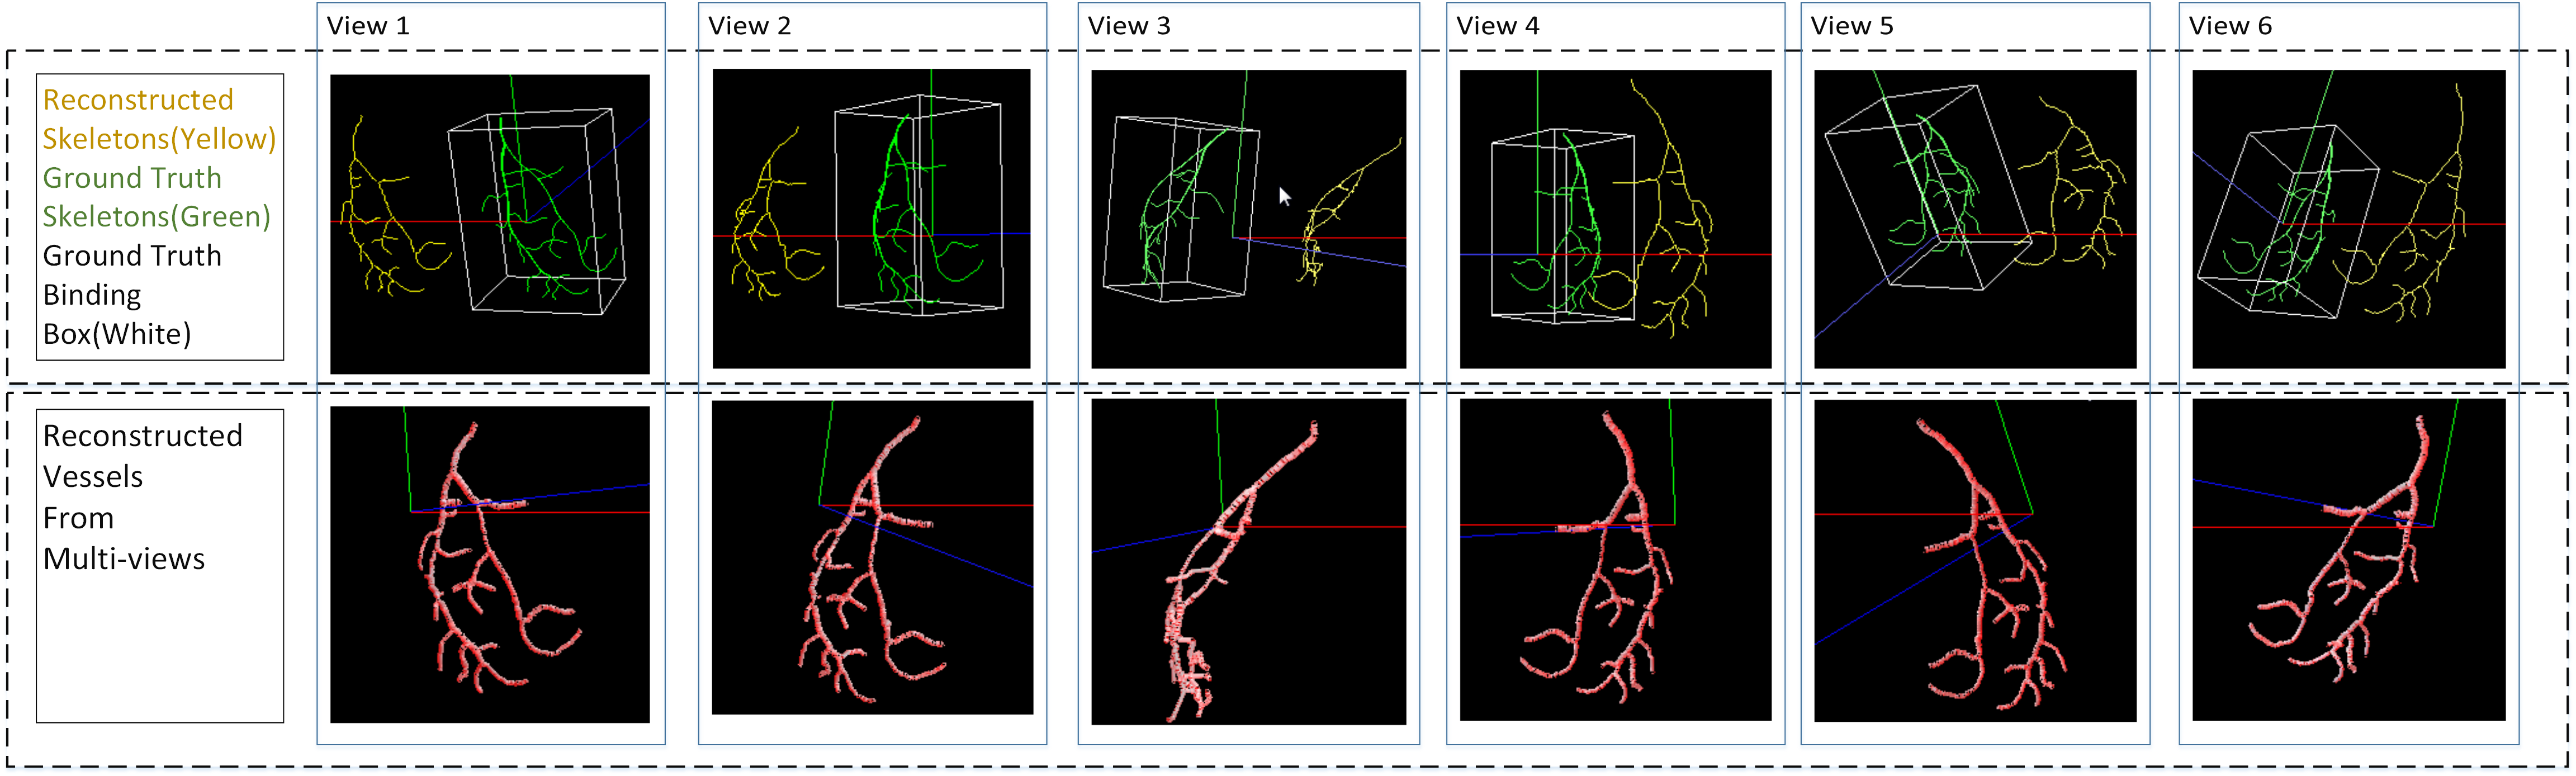
\includegraphics[width=6.0in]{experiments_full.png}\\
  \caption{Up: Reconstructed Centerlines and Ground Truth from Different Views; Down: Reconstructed Vessels}\label{fig:experiments_full}
\end{figure*}

In upper columns of Figure\ref{fig:experiments_full}, the yellow lines
indicate the reconstructed skeleton using our method. The green lines
indicate the ground truth obtained from our simulation platform. The white
box is the binding box of the ground truth. We use the size of the binding
box to evaluate the reconstructed skeletons. We compute the distance between
each ground truth point and the computed point.Then we compute the average
distance as the error. We use the scale the error divides the size of the
binding box to evaluate our reconstructed precision. The error statistics
are described as Figure \ref{fig:error_statistics}.

\begin{figure}
  \centering
  % Requires \usepackage{graphicx}
  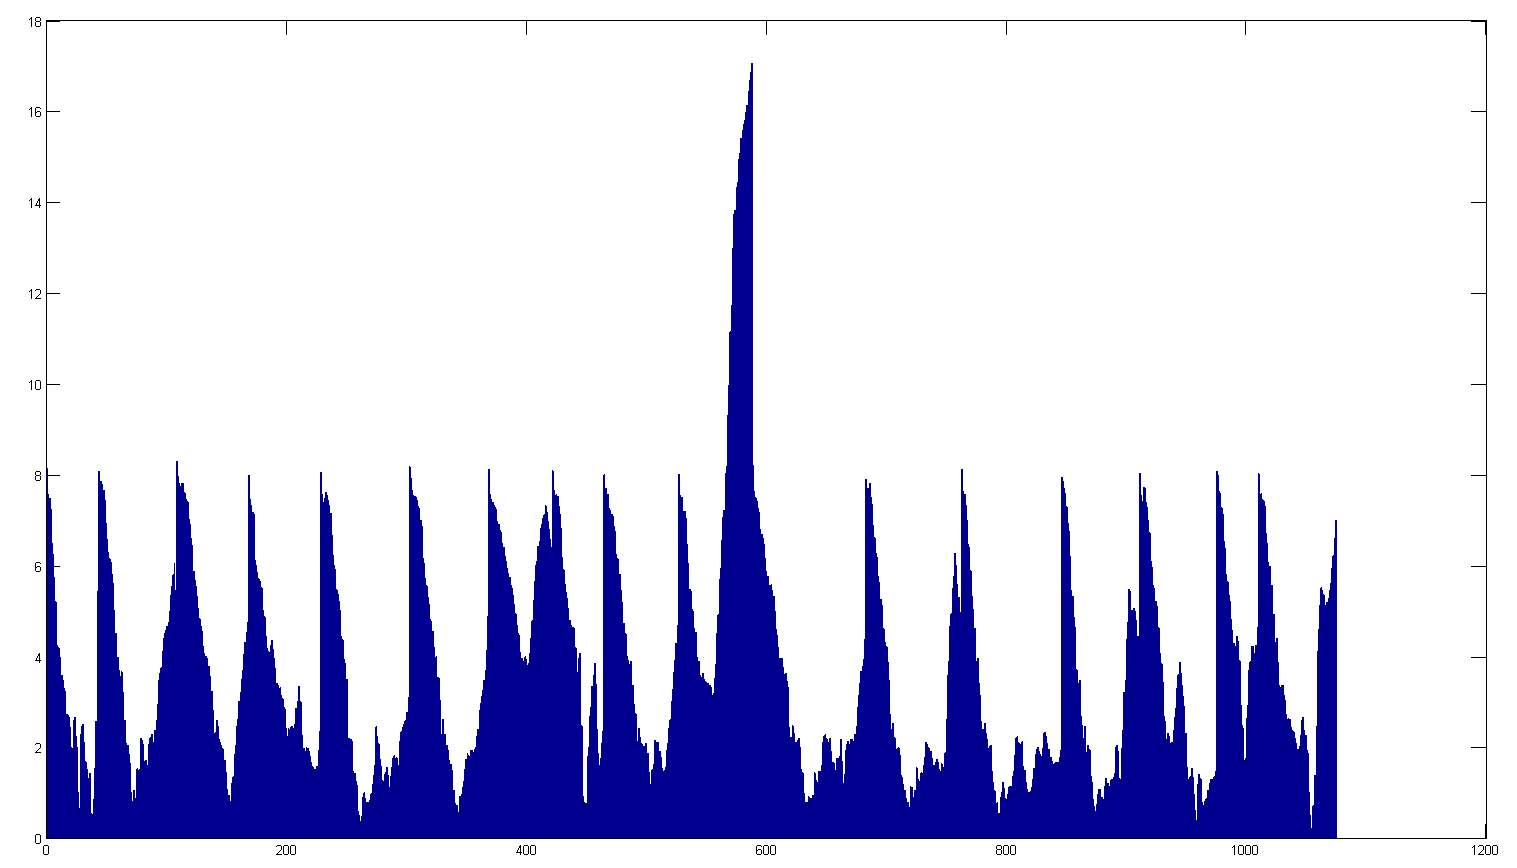
\includegraphics[width=3.0in]{error_statistics.png}\\
  \caption{Error Statistics between Reconstructed Skeletons and Ground Truth}\label{fig:error_statistics}
\end{figure}

Finally, we get an average error of 3.833708 and the binding box of
(52.691906, 77.026981, 39.552235).

As for the real data, the views and reconstructed data can be found in
Figure \ref{fig:real_reconstructed_data}.

\begin{figure}
  \centering
  % Requires \usepackage{graphicx}
  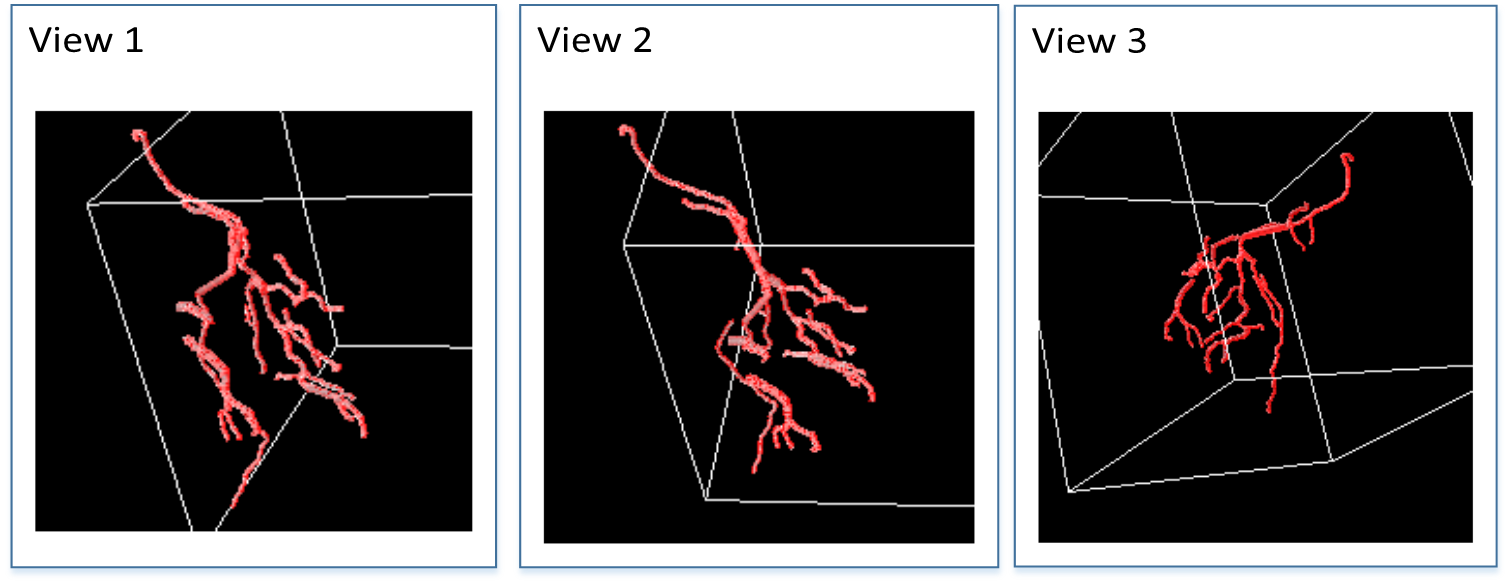
\includegraphics[width=3.0in]{real_data_final.png}\\
  \caption{Reconstructed Real Data}\label{fig:real_reconstructed_data}
\end{figure}

\subsection{Performance}
Our method consists of three steps and the consuming time of each step can
be described in Table \ref{tbl:performance}.

\begin{table}
\begin{tabular}{|c|c|c|c|}
\hline
Step &Called Times&Total Time&Average Time\\
\hline
1 & 57 & 66.024s & 1.158s \\
\hline
2 & 30 & 230.634s & 7.6878s \\
\hline
3 & 1 &27.3s & 27.3s \\
\hline
\end{tabular}
\caption{Step Execution Time}\label {tbl:performance}
\end{table}
Step 1 indicate Vessel Extraction, step 2 indicate Centerline Tracking and
step 3 indicate 3D Reconstruction. According to the table, the centerline
tracking and 3D reconstruction step consumes most time, in our future work,
we wanna implement them on GPU.
